\begin{figure}[H]
    \centering

    \begin{subfigure}[t]{.6\textwidth}
        \centering
        \begingroup
  \sbox{\tempbox}{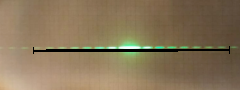
\includegraphics[width=\textwidth]{figuras/medidas/C4.pdf}}
  \begin{picture}(\wd\tempbox,\ht\tempbox)
    \put(0,0){\usebox{\tempbox}}
    \put(.502\wd\tempbox,.33\ht\tempbox){$8~\Delta y$}
  \end{picture}
\endgroup


        \caption{C4}
        \label{fig:C4}
    \end{subfigure}
    \qquad
    \begin{subfigure}[t]{.6\textwidth}
        \centering
        \begingroup
  \sbox{\tempbox}{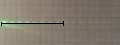
\includegraphics[width=\textwidth]{figuras/medidas/C5.pdf}}
  \begin{picture}(\wd\tempbox,\ht\tempbox)
    \put(0,0){\usebox{\tempbox}}
    \put(.22\wd\tempbox,.38\ht\tempbox){$4~\Delta y$}
  \end{picture}
\endgroup


        \caption{C5}
        \label{fig:C5}
    \end{subfigure}
    \qquad
    \begin{subfigure}[t]{.6\textwidth}
        \centering
        \begingroup
  \sbox{\tempbox}{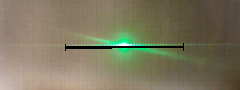
\includegraphics[width=\textwidth]{figuras/medidas/C6.pdf}}
  \begin{picture}(\wd\tempbox,\ht\tempbox)
    \put(0,0){\usebox{\tempbox}}
    \put(.47\wd\tempbox,.39\ht\tempbox){$20~\Delta y$}
  \end{picture}
\endgroup


        \caption{C6}
        \label{fig:C6}
    \end{subfigure}

    \caption{Fotos dos padrões de difração das fendas C}
    \label{fig:C}
\end{figure}